% ============================================================================
% Consciousness Trilogy
% Complete Collected Volume
% Zenodo Upload Edition
% ============================================================================

\documentclass[12pt,a4paper,openany]{book}

\usepackage[utf8]{inputenc}
\usepackage[T1]{fontenc}
\usepackage{amsmath,amssymb,amsfonts,amsthm}
\usepackage{graphicx}
\usepackage[hidelinks]{hyperref}
\usepackage{pdfpages}
\usepackage{geometry}
\usepackage{fancyhdr}
\usepackage{array}
\newcolumntype{P}[1]{>{\raggedright\arraybackslash}p{#1}}
\usepackage{booktabs}
\usepackage{xcolor}
\usepackage{caption}
\usepackage{float}

\geometry{a4paper, margin=1in, headheight=14pt}

\pagestyle{fancy}
\fancyhf{}
\fancyhead[LE,RO]{\thepage}
\fancyhead[RE]{\textit{Consciousness Trilogy}}
\fancyhead[LO]{\textit{\leftmark}}
\renewcommand{\headrulewidth}{0.4pt}

\title{
  \vspace{-2cm}
  {\Huge\textbf{Consciousness Trilogy}}\\[1cm]
  {\Large\textit{Inseparability, Gravity, and the Open\\
  Explanatory Gap}}\\[2cm]
  {\large Complete Collected Volume}\\[0.5cm]
  {\normalsize Papers I, II, and III}
}

\author{
  \textbf{Sidong Liu, PhD}\\[0.5em]
  iBioStratix Ltd\\[0.3em]
  \texttt{sidongliu@hotmail.com}
}

\date{July 2026}

\begin{document}
\emergencystretch=2em
\raggedbottom
\hbadness=5000
\vbadness=5000

\frontmatter
\maketitle

\newpage
\thispagestyle{empty}
\vspace*{\fill}
\begin{center}
\textbf{Publication Record}\\[2em]
\begin{tabular}{ll}
Collected Volume & DOI: 10.5281/zenodo.19608174 \\
\\[-0.2em]
Paper I & DOI: 10.5281/zenodo.19607387 \\
Paper II & DOI: 10.5281/zenodo.19607543 \\
Paper III & DOI: 10.5281/zenodo.19607724 \\
\end{tabular}
\\[3em]
\textit{This collected volume compiles previously published works\\
for archival and reference purposes.}
\\[2em]
\copyright{} 2026 Sidong Liu. All rights reserved.
\end{center}
\vspace*{\fill}

\chapter*{Abstract}
\addcontentsline{toc}{chapter}{Abstract}

This volume collects the three papers of the \emph{Consciousness Trilogy},
an algebraic and information-geometric programme that recasts the hard
problem of consciousness as a question about the independent deformability
of geometric and first-person structural data.

The trilogy develops a three-step logical chain:

\begin{enumerate}
\item \textbf{Paper~I: Inseparability.} Within a Type~III$_1$
algebraic setting, emergent geometry and modular flow are shown not to
be independently deformable. The result is a structural inseparability
theorem, not a reductive identity claim, and the explanatory gap is
relocated from an alleged production failure to the problem of
self-description by finite observers.

\item \textbf{Paper~II: Higher-Dimensional Consistency.} In the CHM
small-ball framework, the higher-dimensional modular datum is identified
as the full family of ball modular Hamiltonians across centers, radii,
and timelike directions. Compatibility with one geometry yields a
conditional leading-order consistency relation in the CHM small-ball
regime; it does not by itself prove a general gravitational uniqueness
claim.

\item \textbf{Paper~III: Open Explanatory Gap.} Finite self-description
is studied through conditional arithmetic self-models. The former local
minimax drift-floor theorem is withdrawn, and the residual explanatory
gap remains open rather than quantitatively closed by a nonzero floor.
\end{enumerate}

Taken together, the three papers propose a coherent programme in which
the hard problem's standard independent-describability presupposition is
not available in the relevant algebraic setting, higher-dimensional
consistency can be analyzed in a CHM local regime, and the remaining
finite self-description gap is explicitly left open.

\bigskip
\noindent\textbf{Keywords}: algebraic quantum field theory, Tomita--Takesaki
modular theory, Guido--Longo--Wiesbrock reconstruction, CHM ball
Hamiltonians, linearized gravity, Fisher information geometry,
self-description, explanatory gap

\tableofcontents

\mainmatter

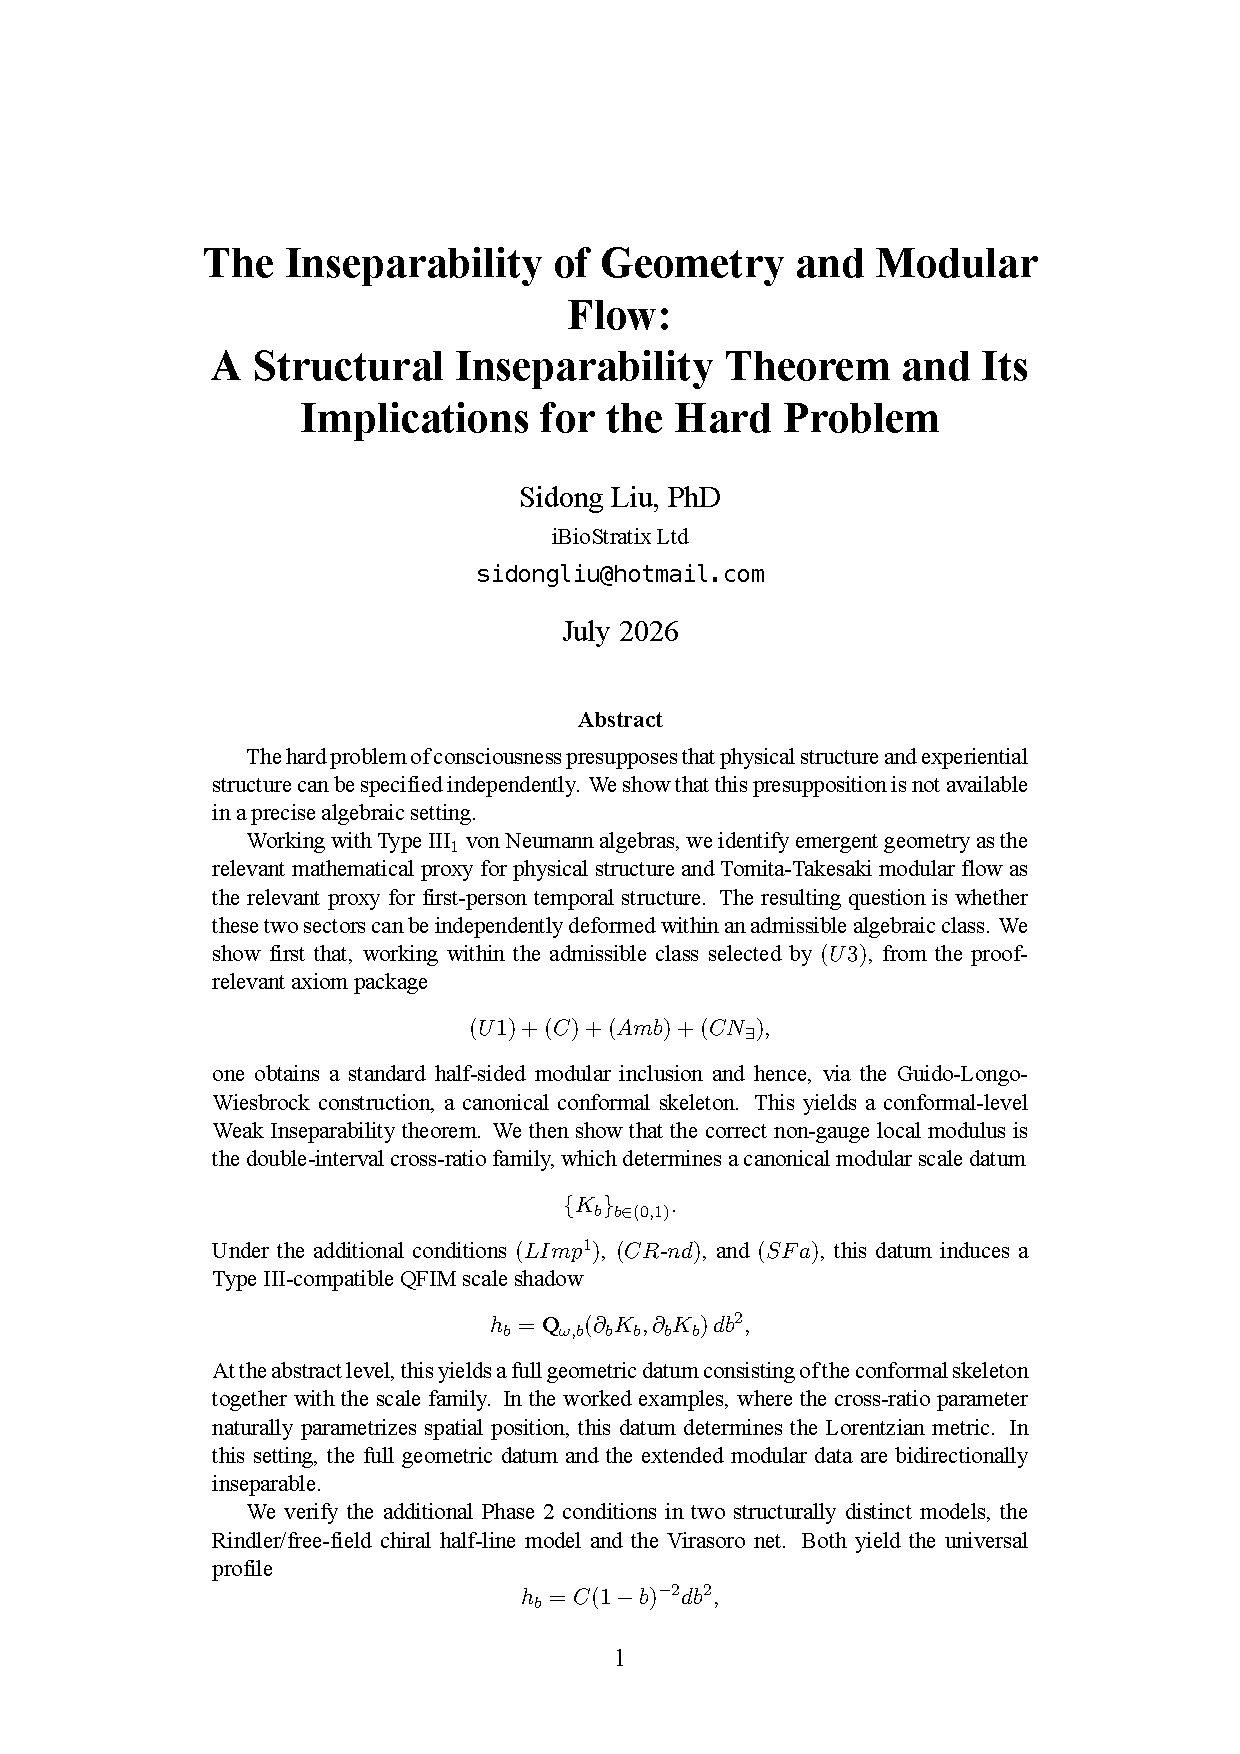
\includepdf[
  pages=-,
  pagecommand={\thispagestyle{empty}},
  addtotoc={1,chapter,1,{Paper I: The Inseparability of Geometry and Modular Flow},chap:paperI}
]{CI_Inseparability.pdf}

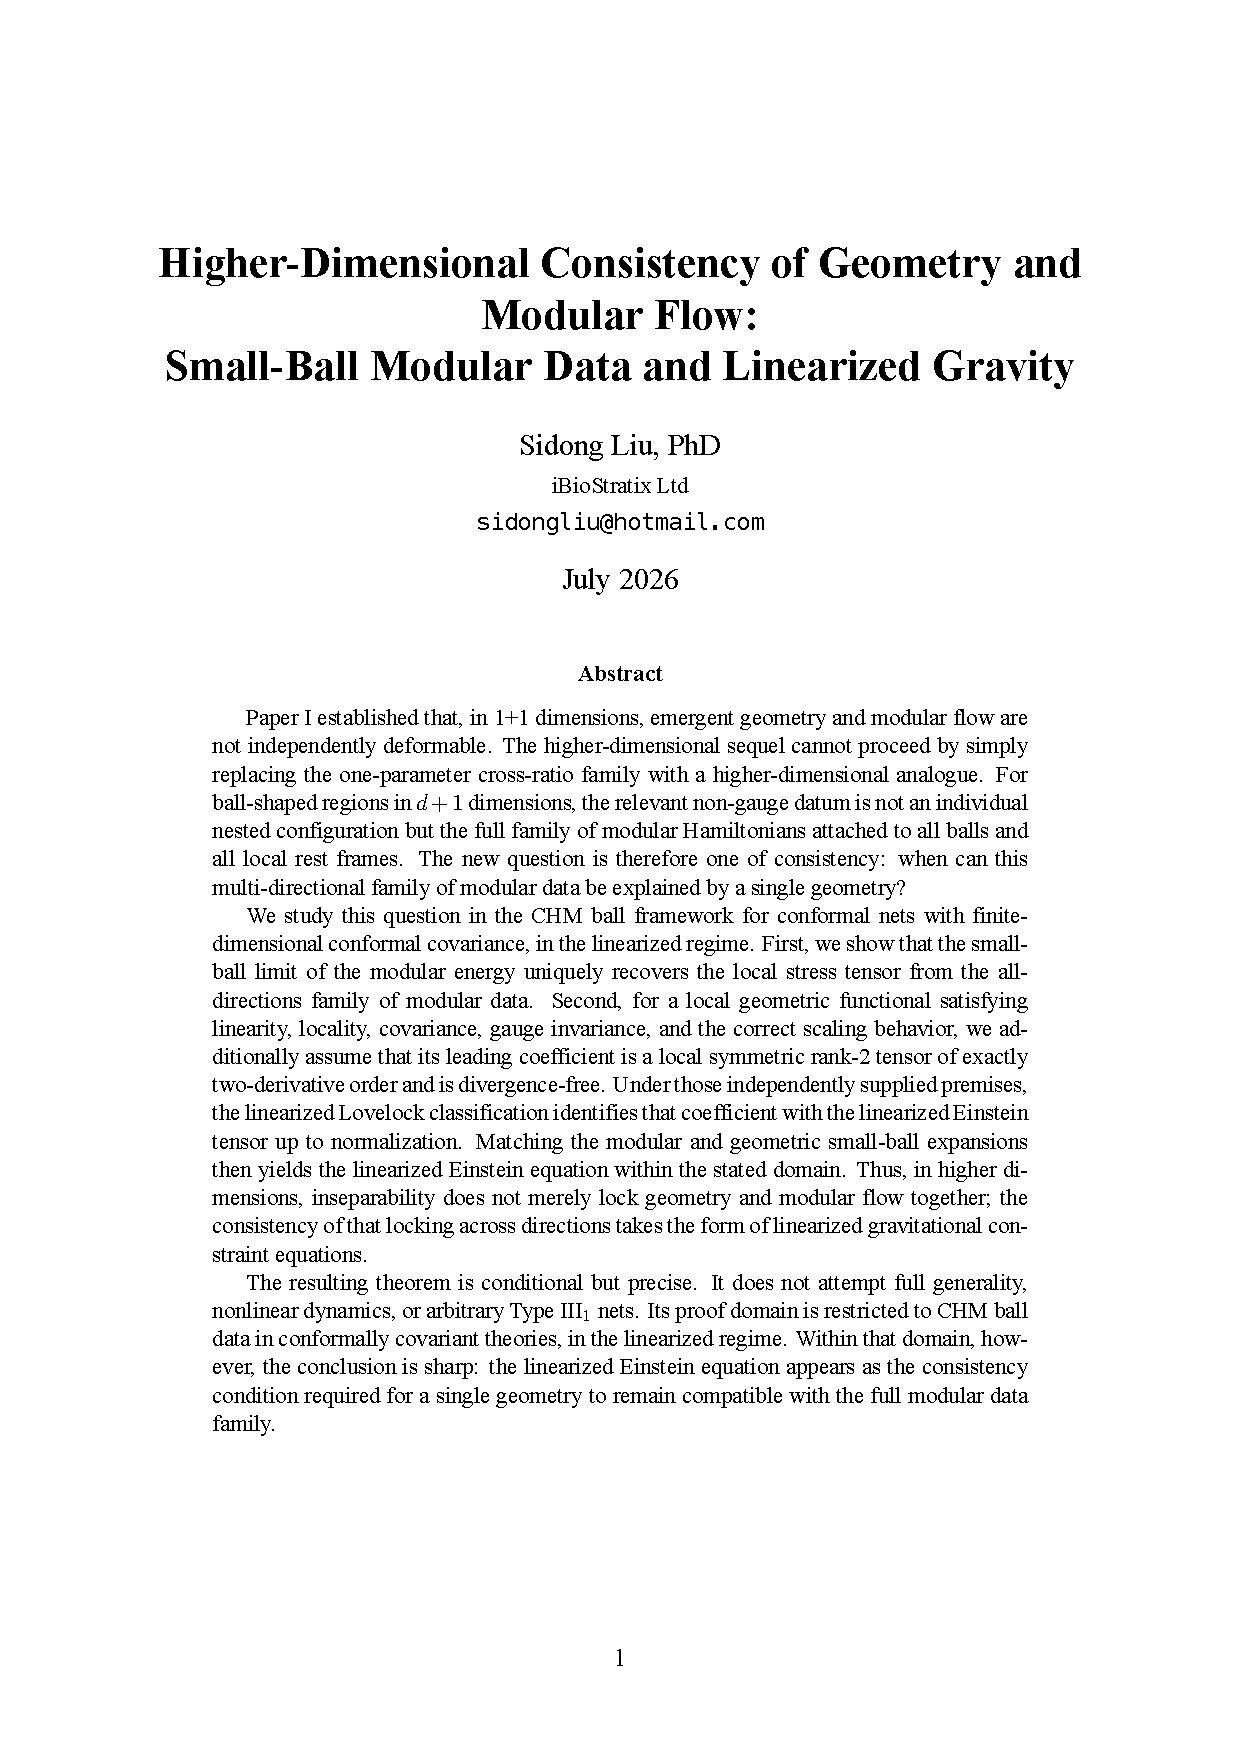
\includepdf[
  pages=-,
  pagecommand={\thispagestyle{empty}},
  addtotoc={1,chapter,1,{Paper II: Higher-Dimensional Consistency of Geometry and Modular Flow},chap:paperII}
]{CII_Higher_Dimensional.pdf}

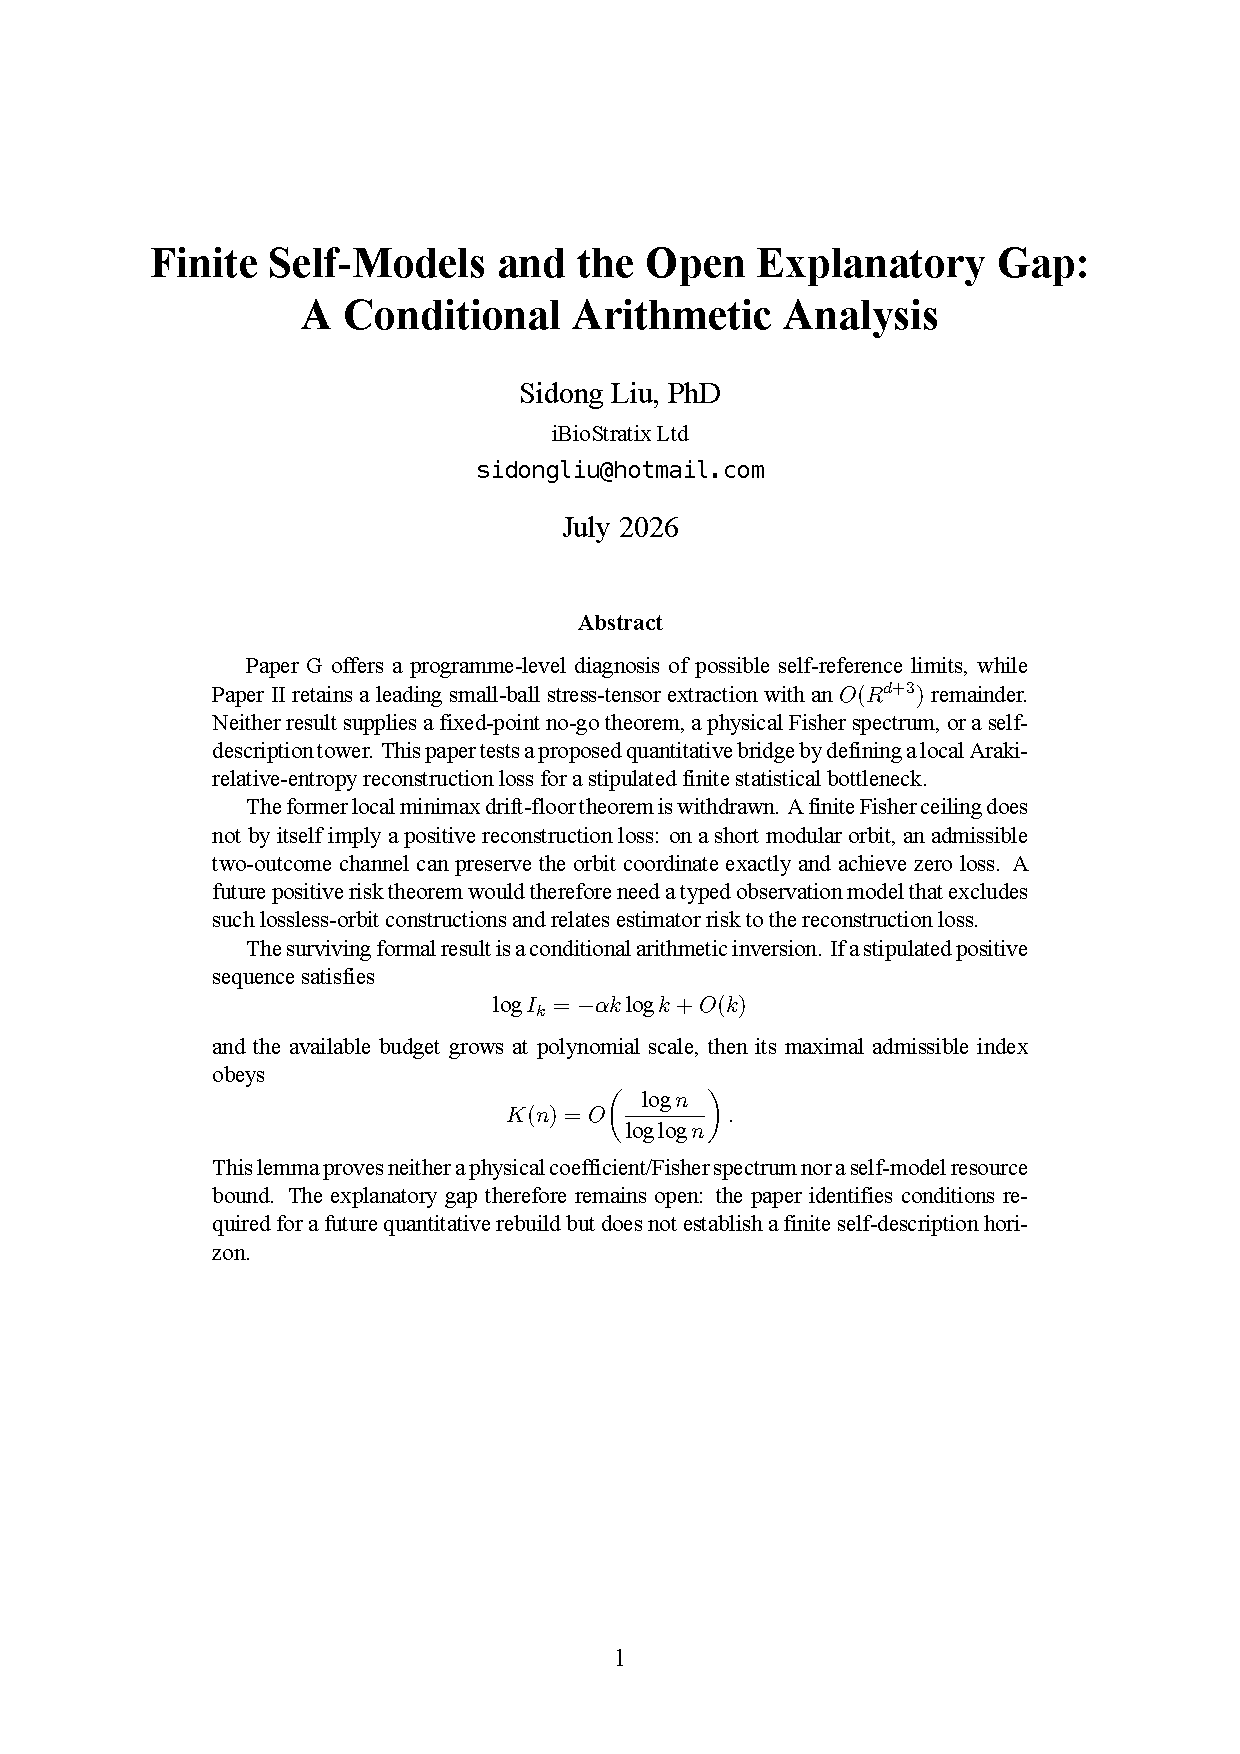
\includepdf[
  pages=-,
  pagecommand={\thispagestyle{empty}},
  addtotoc={1,chapter,1,{Paper III: Finite Self-Models and the Open Explanatory Gap},chap:paperIII}
]{CIII_Finite_Self_Models.pdf}

\end{document}
